\subsection{YOLOv8 Model} \label{subsec:yolo}

\begin{figure}[H]
	\centering
	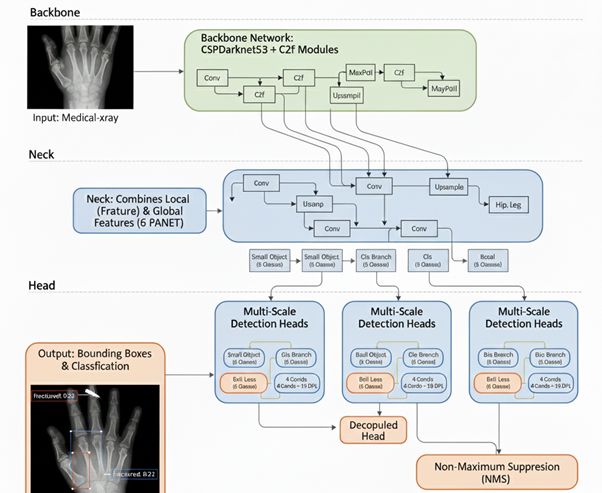
\includegraphics[width=\linewidth]{assets/yolo-arch.png}
	\caption{General architecture of YOLOv8 illustrating the backbone, neck, and detection head components.}
	\label{fig:yolo-arch}
\end{figure}

Object detection has become one of the most important computer vision tasks in modern medical image analysis due to its ability to simultaneously identify and localize pathological findings within an image. Unlike conventional image classification models that only determine whether a disease is present, object detection models additionally provide spatial information regarding the location of abnormalities. This capability is particularly valuable in lung cancer diagnosis, where clinicians must not only determine the presence of a suspicious lesion but also identify its precise location within the lungs.

In the proposed framework, lung cancer detection is formulated as an object detection problem rather than a traditional image classification task. Instead of predicting a single label for an entire CT scan, the model identifies suspicious cancerous regions and generates bounding boxes surrounding them. To accomplish this task, the proposed system employs YOLOv8 (You Only Look Once Version 8), one of the most recent and advanced members of the YOLO family of object detection architectures.

YOLOv8 is a single-stage object detector, meaning that object localization and classification are performed within a single forward pass through the network. This design significantly reduces computational complexity compared to two-stage detectors such as Faster R-CNN, which first generate candidate regions and subsequently classify them. By combining both operations into a unified architecture, YOLOv8 achieves high detection accuracy while maintaining efficient inference speeds. These characteristics make it particularly suitable for deployment within real-time clinical decision support systems where rapid analysis of CT scans is desirable.

The complete processing pipeline employed by the proposed lung cancer detection model is illustrated in Figure~\ref{fig:yolo_pipeline}.

\begin{figure}[H]
	\centering
	
	\resizebox{\linewidth}{!}{
		\begin{tabular}{c c c c c c c c c c c}
			\fbox{
				\begin{tabular}{c}
					Chest CT\\
					Input
				\end{tabular}
			}
			&
			$\rightarrow$
			&
			\fbox{
				\begin{tabular}{c}
					Image\\
					Preprocessing
				\end{tabular}
			}
			&
			$\rightarrow$
			&
			\fbox{
				\begin{tabular}{c}
					YOLOv8\\
					Backbone
				\end{tabular}
			}
			&
			$\rightarrow$
			&
			\fbox{
				\begin{tabular}{c}
					PANet\\
					Neck
				\end{tabular}
			}
			&
			$\rightarrow$
			&
			\fbox{
				\begin{tabular}{c}
					Detection\\
					Head
				\end{tabular}
			}
			&
			$\rightarrow$
			&
			\fbox{
				\begin{tabular}{c}
					Lung Cancer\\
					Detection
				\end{tabular}
			}
		\end{tabular}
	}
	
	\caption{End-to-end processing pipeline of the proposed YOLOv8 lung cancer detection model.}
	\label{fig:yolo_pipeline}
\end{figure}

As illustrated in Figure~\ref{fig:yolo-arch}, YOLOv8 consists of three primary components: the backbone, the neck, and the detection head. Each component contributes a specific functionality to the overall detection process.

\subsubsection{Backbone Network}

The backbone serves as the feature extraction component of YOLOv8. Its primary objective is to transform raw CT scan images into hierarchical feature representations that can be used for lesion detection. YOLOv8 employs the C2f (Cross-Stage Partial Bottleneck with Two Convolutions) architecture, which is an evolution of the CSP (Cross Stage Partial) designs used in previous YOLO versions.

The backbone progressively applies convolutional operations to the input image, generating increasingly abstract feature maps. Early layers learn low-level visual characteristics such as edges, gradients, and texture variations, while deeper layers capture more complex semantic information associated with pulmonary nodules, masses, and abnormal tissue structures.

One of the key advantages of the C2f architecture is its ability to improve gradient propagation while reducing computational overhead. By reusing features across multiple layers, the network can learn richer representations without requiring excessive numbers of parameters. This characteristic is particularly beneficial in medical imaging applications where datasets are often smaller than those available in general computer vision tasks.

For lung cancer detection, the backbone learns to distinguish subtle visual differences between healthy lung tissue and suspicious lesions. These differences may include variations in density, texture, shape, and intensity patterns that are characteristic of malignant abnormalities.

\subsubsection{Neck Network}

The neck component is responsible for feature aggregation and multi-scale feature fusion. In YOLOv8, this functionality is implemented using a Path Aggregation Network (PANet).

Feature extraction layers at different depths of the backbone capture information at different scales. Shallow layers retain detailed spatial information, while deeper layers capture more abstract semantic features. Because lung cancer lesions can vary significantly in size, relying on a single feature scale would limit detection performance.

Small pulmonary nodules may occupy only a tiny portion of the CT image, whereas larger tumors may extend across substantial regions of the lung. The PANet structure addresses this challenge by combining feature maps generated at multiple scales. Through repeated top-down and bottom-up information flow, PANet enables the model to simultaneously utilize local texture details and broader anatomical context.

Consequently, the neck allows YOLOv8 to detect both small and large lesions while maintaining accurate localization performance across a wide range of tumor sizes.

\subsubsection{Detection Head}

The final component of YOLOv8 is the detection head. This module is responsible for generating the actual predictions produced by the network.

Unlike earlier object detectors that relied on predefined anchor boxes, YOLOv8 employs an anchor-free detection strategy. Rather than predicting offsets relative to predetermined anchors, the model directly predicts object centers and bounding box coordinates.

The detection head performs two independent tasks:

\begin{itemize}
	\item Classification of detected regions.
	\item Localization of detected lesions.
\end{itemize}

This decoupled architecture allows each task to be optimized independently, improving overall detection performance. For each detected region, the model predicts:

\begin{itemize}
	\item Bounding box coordinates.
	\item Object confidence score.
	\item Cancer detection probability.
\end{itemize}

The resulting predictions are then forwarded to the post-processing stage for refinement.

\subsubsection{Multi-Scale Detection}

A major challenge in lung cancer detection is the substantial variability in lesion size. Early-stage tumors may appear as extremely small nodules, whereas advanced-stage tumors can occupy large portions of the lung field.

YOLOv8 addresses this challenge through multi-scale detection. Detection heads operate on feature maps of different resolutions, enabling the model to identify abnormalities across multiple spatial scales.

This capability is particularly important in CT-based diagnosis because the early detection of small nodules is often critical for improving patient outcomes. Multi-scale processing allows the model to preserve fine-grained details while simultaneously leveraging high-level semantic information extracted from deeper network layers.

The full process of multi-scale feature extraction is shown in Figure~\ref{fig:yolo_multiscale}

\begin{figure}[H]
	\centering
	
	\begin{tabular}{ccc}
		
		\fbox{
			\begin{minipage}{0.25\textwidth}
				\centering
				High-Resolution Features\\
				(Small Nodules)
			\end{minipage}
		}
		
		&
		
		\fbox{
			\begin{minipage}{0.25\textwidth}
				\centering
				Medium-Resolution Features\\
				(Intermediate Lesions)
			\end{minipage}
		}
		
		&
		
		\fbox{
			\begin{minipage}{0.25\textwidth}
				\centering
				Low-Resolution Features\\
				(Large Tumors)
			\end{minipage}
		}
		
	\end{tabular}
	
	\vspace{0.5cm}
	
	$\downarrow$
	
	\vspace{0.3cm}
	
	\fbox{
		\begin{minipage}{0.4\textwidth}
			\centering
			Unified Multi-Scale Detection Output
		\end{minipage}
	}
	
	\caption{Multi-scale feature extraction employed by YOLOv8 for detecting lung lesions of varying sizes.}
	\label{fig:yolo_multiscale}
\end{figure}

\subsubsection{Anchor-Free Detection Mechanism}

Traditional object detection models rely on predefined anchor boxes that attempt to approximate the expected shapes and sizes of target objects. Although effective in many applications, anchor-based methods introduce additional hyperparameters and often struggle with irregularly shaped objects.

Lung tumors exhibit substantial variability in morphology and rarely conform to standardized geometric patterns. Consequently, anchor-based approaches may fail to adequately represent their boundaries.

YOLOv8 addresses this limitation by adopting an anchor-free detection strategy. Instead of matching objects to predefined anchor templates, the model directly predicts object centers and corresponding bounding box coordinates.

This design offers several advantages:

\begin{itemize}
	\item Reduced hyperparameter complexity.
	\item Improved adaptability to irregular tumor shapes.
	\item Faster convergence during training.
	\item Enhanced localization performance.
\end{itemize}

These characteristics make anchor-free detection particularly suitable for medical imaging applications involving heterogeneous pathological structures.

\subsubsection{Bounding Box Regression and Localization}

Once suspicious regions have been identified, YOLOv8 must determine the exact boundaries of each lesion.

Bounding box regression is performed by predicting:

\begin{itemize}
	\item Horizontal position.
	\item Vertical position.
	\item Width.
	\item Height.
\end{itemize}

These predictions are continuously refined throughout training using specialized localization loss functions. The resulting bounding boxes provide interpretable visual evidence regarding the location of suspicious findings and can assist clinicians during diagnostic review.

\subsubsection{Non-Maximum Suppression}

Object detectors frequently generate multiple overlapping predictions for the same lesion. To eliminate redundant detections, YOLOv8 employs Non-Maximum Suppression (NMS).

The process is illustrated in Figure~\ref{fig:yolo_nms}.

\begin{figure}[H]
	\centering
	
	\resizebox{0.95\linewidth}{!}{
		\begin{tabular}{c c c c c c c}
			
			\fbox{
				\begin{tabular}{c}
					Overlapping\\
					Bounding Boxes
				\end{tabular}
			}
			
			&
			$\rightarrow$
			&
			
			\fbox{
				\begin{tabular}{c}
					IoU\\
					Calculation
				\end{tabular}
			}
			
			&
			$\rightarrow$
			&
			
			\fbox{
				\begin{tabular}{c}
					Non-Maximum\\
					Suppression
				\end{tabular}
			}
			
			&
			$\rightarrow$
			&
			
			\fbox{
				\begin{tabular}{c}
					Final Lung Cancer\\
					Detection
				\end{tabular}
			}
			
		\end{tabular}
	}
	
	\caption{Non-Maximum Suppression procedure used to remove duplicate detections and retain the highest-confidence prediction.}
	\label{fig:yolo_nms}
\end{figure}

The overlap between predicted and ground-truth boxes is measured using the Intersection over Union (IoU) metric:

\[
IoU =
\frac
{
	Area(B_p \cap B_g)
}
{
	Area(B_p \cup B_g)
}
\]

where \(B_p\) denotes the predicted bounding box and \(B_g\) denotes the ground-truth bounding box.

Predictions with excessive overlap are suppressed, ensuring that each lesion is represented by a single final detection.

\subsubsection{Training Objective and Loss Functions}

YOLOv8 optimizes a composite loss function composed of multiple components.

\paragraph{Classification Loss (Binary Cross-Entropy)}

Binary Cross-Entropy loss guides the model in distinguishing cancerous lesions from background regions. This loss encourages accurate classification while minimizing false positive detections.

\paragraph{Box Localization Loss (CIoU)}

Complete Intersection over Union (CIoU) loss evaluates localization quality by considering overlap area, center distance, and aspect ratio differences between predicted and ground-truth boxes.

This loss can be expressed conceptually as:

\[
L_{CIoU}
=
1 - IoU
+
\text{Distance Penalty}
+
\text{Aspect Ratio Penalty}
\]

where additional penalty terms improve localization precision.

\paragraph{Distribution Focal Loss (DFL)}

Distribution Focal Loss improves boundary estimation by modeling uncertainty in bounding box coordinates. This is particularly important in medical images where lesion boundaries may be ambiguous or partially obscured.

Together, these loss functions allow YOLOv8 to simultaneously optimize classification accuracy and localization quality.

\subsubsection{Suitability of YOLOv8 for Lung Cancer Detection}

Several characteristics make YOLOv8 particularly suitable for lung cancer detection.

First, its single-stage architecture provides rapid inference speeds while maintaining high detection accuracy. This allows the model to be integrated into real-time diagnostic support systems.

Second, multi-scale feature extraction enables the detection of lesions exhibiting substantial size variation, ranging from small pulmonary nodules to larger malignant masses.

Third, the anchor-free detection mechanism improves adaptability to irregular tumor morphologies commonly encountered in clinical practice.

Fourth, the generated bounding boxes provide intuitive visual explanations that can assist clinicians in understanding and verifying model predictions.

Finally, YOLOv8 benefits from transfer learning, allowing knowledge acquired from large-scale image datasets to be leveraged for medical imaging tasks. This capability is especially valuable when working with limited annotated medical datasets.

To evaluate the effectiveness of the proposed lung cancer detection model, Precision, Recall, and mAP50 are employed as the primary performance metrics. Precision quantifies the proportion of detected lesions that are truly cancerous, Recall measures the proportion of actual lesions successfully identified by the model, and mAP50 provides a comprehensive assessment of overall detection performance by evaluating both localization and classification accuracy at an Intersection over Union threshold of 0.50.

Collectively, these metrics provide a rigorous evaluation of the model's ability to accurately identify and localize lung cancer lesions within chest CT scans, ensuring that the resulting system can serve as a reliable component of the proposed intelligent diagnostic framework.